\documentclass[sigconf]{acmart}

\usepackage{graphicx}
\usepackage{hyperref}
\usepackage{todonotes}

\usepackage{endfloat}
\renewcommand{\efloatseparator}{\mbox{}} % no new page between figures

\usepackage{booktabs} % For formal tables

\settopmatter{printacmref=false} % Removes citation information below abstract
\renewcommand\footnotetextcopyrightpermission[1]{} % removes footnote with conference information in first column
\pagestyle{plain} % removes running headers

\newcommand{\TODO}[1]{\todo[inline]{#1}}

\begin{document}
\title{Agricultural Data Science: Then, Now, and Beyond}


\author{Ross Wood}
\affiliation{HID345}
\email{rmw@indiana.edu}

\begin{abstract}

As the human population swells to staggering numbers that historians of yesteryear could not imagine, one very important question seems to keep coming up over and over again. How do we feed all of these people? Thankfully, humans are intelligent beasts and are figuring out ways to farm and produce larger amounts of food using methods and techniques more sophisticated than ones humanity has relied on in the past. The party is just getting started as farming meets the era of big data. As more and more data is generated from farming, techniques and processes become more sophisticated, cleaner, and more efficient. The kind of data being analyzed to improve agricultural endeavours comes in many forms, and can be statistical data like amount of food grown using how much land, actual data generated from using farm tools and other smart farming equipment, or any other kind of agricultural activity that can produce datafies actions and procedures. However, data science is helping in other ways, too, as scientists and engineers are taking advantage of all this newly available data and helping create new technology to improve food production and increase yields  With all this new information available, new farming endeavours are being undertaken. Farming within closed systems such as urban or vertical farming, practicing precision agricultural techniques, or even laboratories using genetics data on different plant strains to crossbreed the various plant strains in order to produce new breeds that can grow in the harshest of environments while using minimal resources. As the population grows, we are finding that not only is the production of food vital, but also that sustainable farming techniques are of paramount importance for long term agricultural need. Data Science and its applications are most definitely changing the way people produce food and the very nature of farming itself.

\end{abstract}

\keywords{i523, HID345, Agricultural Data Science, Smart Farming, Vertical Farms, Urban Farming, Big Data Farming, Smart Farming Tools, Precision Agriculture}

\maketitle

\section{Introduction}

Humans have not always lived in the amazing concrete and technological jungles that we have surrounded ourselves with today. Indeed, the ability to stop being nomadic and settle down in one area is a relatively new development in regards to the grand scale of human existence. However, if there is one technological advancement which is considered to be the most directly responsible for allowing humans to change how they lived and thrive in a harsh and unforgiving world, it would be when ancient humans evolved into the first agrarian societies by figuring out how to plant crops and grow food. By making their societies agriculture based instead of hunting based, humans were able to live in one place and do a lot of gathering, in addition to the hunting they were used to. This regular supply of food and less dependency on hunting allowed ancient humans time to develop other aspects of human society, such as language, writing, and building.  This was about 12,000 years ago and ever since that time, humanity has been gathering data on farming and slowly but surely refining the techniques we use for food production. Humanity has not just been gathering data and knowledge on how to grow food, but also information on what kinds of crops to grow when and where, how to deal with insect, rodent, and pests and other external threats to crops, and how what to do and how to manage different weather and environmental setbacks. These are a few of the many examples of information that humanity has accumulated over the millennia that have allowed humans to improve their farming and agricultural techniques, which has enabled humanity to thrive around the world.

The advances humans have made in their early years of farming will pale in comparison to the advances that humanity has the potential to make in the modern era using big data analytics and sophisticated technology that improves farming methods. With population statistics indicating that there is no sign of our population growth slowing down, the question is becoming even more relevant today than it has been in the past. With estimates putting the world population at 11.2 billion by the year 2100, solving the hunger problem is imperative \cite{green2005}. Using data science and modern data analysis techniques and models, humans are able to look at the concept of agriculture as a whole and start making decisions based on data that had never been readily available in the past. This data is useful to farmers and serves as kind of risk management system through which farmers can make informed decisions about changes they might want to implement on their farms. The rise of smart farming with a focus on sustainability, the ability to analyze information in ways not possible in the past, and the invention of tools like monitoring sensors and machines that datafie work are changing agriculture for the better. The desire for more efficiency, greater food production, and meeting the demands of a steadily growing population are the driving forces behind why this field continues to be researched and expanded. Closed farms that eliminate the need for pesticides and rodenticide use while also helping the environment by cleaning the air in urban areas are a couple of unique ways this field has branched off from traditional farming practices and techniques.

Modern technology and data science are making new agricultural endeavours possible in ways that previously could not have been attempted with any hope of such success modern farmers are finding. One new technique is called urban, or vertical farming. A vertical farm is a farm constructed in an urban area that goes up instead of out. Ideally built in a parking garage like structure, vertical farms use data analysis to make their crop yields extremely efficient. There are plans for their construction coming up in more and more cities over the next couple decades and they are already beginning to appear in developing nations that have problems meeting the demand for fresh fruits and vegetables in major urban centers. Other examples of how data science is changing the agriculture game is through the invention of more sophisticated computer software and languages that allow for the analysis of farming and crop data in ways that could never have been done in the past. This new way of looking at growing, storing, and transporting food and agricultural goods is making humanity second guess a lot of the ways we used to do things with regard to food. The explosive growth of big data and the rise of data science are already changing the way the world works and how we go about our daily lives. Data science is already improving agricultural endeavours in a myriad of ways, just like it does in most fields that it used to solve problems in. The positive benefits of this transition to new approaches in agriculture are already beginning to be seen.

\section{Historical Agricultural Data Science}

The rise of big data analytics software and technology was the turning point where society began to really be able to take advantage of the ever growing amounts of data being produced by farms and their workers. As computer components began to get smaller, cheaper, and more powerful, this enabled more wide spread use of data analysis to be performed, which made it easier for companies and other organizations to adopt these new techniques and get in on the ground floor of solving agricultural problems and changing the way people farm around the world. Despite all these positive steps happening in the fields of technology, data analysis, and data creation, only small groups of people, usually limited to college university campuses, were actually receiving funding to analyze agricultural research data. This lack of funding meant that, although models for agricultural analysis were being developed, they were not being improved upon, leaving the power of data science in the field of agriculture unrealized until it could be adopted by more people and organizations \cite{jones2017}. 

\subsection{Early Agricultural Analysis}

In early to mid 1950s, computers and funding were still only available mostly at universities, which meant that universities were where most data analysis was being done in that era. Despite this, great steps were still being made to lay the foundation of modern agricultural data science and all that that encompasses. From the mid 1950s and onward, modeling was done by various institutions to find things like best water balance, photosynthesis and growth statistics, models to evaluate land and zoning properties, and pinning down economic risk management models, to name a few \cite{jones2017}. These models acted as guidelines and risk management tools in food production decisions making processes. As the availability and use of modeling technology became more widespread and more people and organizations began adopting them, so too did their positive impact on the real world become more apparent and visible. The changes, technological advances, and new techniques that were being proposed to farmers may have been met with some skepticism at first, but by the mid 1970s, these new processes were reportedly responsible for saving the lives of billions of people around the world by helping aid world hunger relief efforts. Like dominoes falling, this led to increases in funding, which led to better and more accurate models being developed, which led to even more advances, which led to more funding, and so on. This self sustaining cycle of budget increases and technological innovation at the beginning of the agricultural data science boom led to the development of new ways of thinking about growing food and led to the development of tools that are still used today. These agricultural systems were developed for many reasons, but the top three reasons they are developed are typically ``the intended use of the model, approaches taken to develop the models, and their target scales`` \cite{jones2017}. Whatever their intent for development, very quickly it was evident that the proof was in the pudding.

\subsection{New Tools for Agricultural and Risk Modeling}

One data analysis tool for statistical decision making that was developed during the early days of agricultural data analysis was a software called Statistical Analysis System, or SAS for short. SAS was developed and ``started out as a tool for statisticians: Goodnight originally developed it to analyze agricultural-research data in North Carolina'' \cite{jones2017}. The development and utilization of SAS made sifting through the piles of random agricultural data much more manageable, and helped proto-data scientists find patterns, make connections, and gleam wisdom from the available agricultural data that they would not have been able to find without using SAS. Being able to manipulate and understand all the available data gave the farmers and data scientists a statistical edge when making choices about changing their farming practices. Economic risk management models would later be developed which helped make farmers more knowledgeable and able to hedge their bets whenever they were attempting new processes and techniques for improving their crops and growing capacity \cite{rose2016}. All of these new models made it easier for farmers to make decisions about making changes in how they produced their crops. The ability to make informed decisions about potentially big changes made farmers less reticent to try new approaches to farming and different techniques in how they produced their crops.

Since the development and implementation of SAS, other techniques have been developed to help take the pressure off of farmers when making educated and informed decisions. Commonly referred to as decision support tools, they have been developed to help farmers and data scientists make heads or tails of all the data that their trade is generating on a day to day basis. Thanks to the development of these kinds of tools and models and their improvement over the years, the decades since their adoption by farmers have seen farms produce more food per acre and increase their own sustainability for the years to come. These tools are incredibly useful to farmers, and ``lead users through clear steps and suggest optimal decision paths or may act as information sources to improve the evidence base for decisions'' \cite{rose2016}. These tools were slow to be developed because of funding problems, but once they began to catch on, they were quickly adopted by farmers to help improve their yields. A statistical analysis of farmers and the tools they used found that the odds of using decision support tools and software increased greatly depending on the size of the farm. The bigger the farm, the better the chances are that they use some kind of decision support tools software \cite{rose2016}. The growth of urbanization and major cities meant that there were less farmers, which means that the farms that did exist were becoming bigger and bigger to fill the vacuum. Larger farms led to more widespread of adoption of the then modern technology and approaches to increase yields, improve efficiency, and improve farming conditions and overall food production.

\subsection{Food Explosion, Courtesy of Data Science}

Slowly but surely, the world, and especially developing nations, began to see the effects of applied data science to agricultural and farming endeavours. It was in the 1960s that a kind of critical mass was reached where the benefits of this field became undeniable. This led to the eventual development of precision farming with a focus on sustainability. All of these new breakthroughs in environmental science helped plant the seeds for what would be the growing environmental movements. In the mid to late 20th century, scientists like Norman Borlaug, who would later win a Nobel Peace Prize for his research, pioneered the way in using analysis models on plant genetics in order to improve yield by finding which breeds were best to cross and grow in different environments. These experiments led directly to the development of high yield crops in 1960s Mexico, and would later do the same in India \cite{borlaug2007}. Analysis of crop data allowed for the scientist to breed genetically superior strains of cereal grains that could withstand harsher climates, thrive on fewer resources like water and fertilizer, and produce a greater yield per acre than strains that Mexican farmers had previously been using. These new strains were potent and unlike anything the world had ever seen. When the Mexican farmers adopted these strains that Borlaug and his team had developed, they immediately began to see an improvement in their ability to meet the food demand of their population. While not alleviating the problem of hunger entirely, these developments proved that applying data science solutions to agricultural problems yields great results. These developments helped stymie off a hunger epidemic, and when Borlaug received his Nobel Peace Prize in 1970, it was officially for ``saving over a billion lives'' \cite{borlaug2002}. This quick turnaround showed definitively that research and development in agricultural data science was worth the investment, as less than 25 years after these new processes and models were being worked out, they were able to be used to save billions of lives.

These achievements, fantastical as they may be, only helped stymie off the threat of hunger around the world temporally, as these kinds of advances could only go so far. Growing populations steadily defeat advancements in food production, and humanity has to keep adapting and refining our methods and techniques in order to continually meet the needs of the many \cite{mendelsohn1999}. Luckily, humans are clever creatures, and our innovation and technological achievements have grown exponentially with our massive populations. More powerful computers and data analysis methods are constantly making humans better at producing food and meeting the staggering population demands. The gradual advance in sophistication of humankind's ability to produce food and knowledge of best techniques and practices continues to evolve with technology and available data. Data science is just the newest and sharpest tool in humanity's toolbox and its use is improving farming in every way.


\subsection{The End of the Past}

History is a gradual process which only seems instantaneous when reading about it in a history book. When talking about agricultural data science and its past, present, and future, it would be easier to think about it like stepping stones. The future did not just come to be, but contributions from the farmers and data scientists in the past helped to build it up to where it is today. But which stepping stones are the most important ones to be looking at when thinking agricultural data science's past? Ultimately, the best example the past can provide is that working together and openly is the most beneficial approach for everyone involved.

Some of the biggest developments from the 20th century of agriculture came about because of the open nature of the field, but there were other circumstances that led to great leaps in agricultural data science. Other circumstances that have led to advances in this field are: 1) the ability to capitalize on a crisis, 2) advances in technology and hardware, 3) keeping the data open and harmonized, 4) making the data easily applicable so that it can be used in other disciplines, 5) developing and maintaining standards and protocols, and 6) making sure the data remains user friendly and user-driven \cite{jones2017}. These approaches represent ideal ways to handle and manage agricultural data so that it can be used and expanded upon by all parties that might be interested. Keeping the data open allows for greater innovation as it becomes a problem that is solved on a societal level, not an individual one. This helps keep the data user friendly and driven as well. All of these different examples represent the various stepping stones that have worked together to bring the field of agricultural data science from its roots in human history and changes in the 20th century, to the modern way we look at agriculture and farming in the 21st century.

\section{Modern Agricultural Data Science}

In the 21st century, humanity has the hindsight to know that data science and its endeavours yield their own rewards. As a result, funding for the study of agricultural endeavours using data science is no longer too difficult to come by. The different areas under the umbrella that is agricultural data science have, in many ways, become fields unto themselves. Urban and precision farming, networked farms, and agricultural technological innovation all have their own sub-fields, but they all belong to the field of agriculture data science in one way or another. All of these different fields that make up modern agricultural data science have one attribute in common, however, and that one attribute is a focus on sustainability in whatever agricultural endeavour that is being undertaken. Indeed, modern data scientists and farmers would have a difficult time encouraging and practicing new processes that did not take sustainability into account. With the world's population expected to keep growing, and the amount of food needed to feed the population expected to double by 2050 \cite{green2005}, this new focus on sustainability is an ever growing piece of the modern farming puzzle, whose importance and juxtaposition along side traditional and modern beliefs about agriculture can no longer afford to be overlooked. Data science factors into this tremendously as it enables farmers and agriculturalists to analyze their data and figure out if their new approaches and techniques are actually working and worth continuing.

Focusing on sustainability and changing things around the farm are not the only new tricks that modern farmers and data scientists have up their sleeves. New techniques and advances in computing technology, both hardware and software, have helped pave the way towards making the analysis of farming data easier and more available than ever so that farmers and agriculturalists can make informed decisions about how they grow their crops and produce food. One example of a new technique that has been developed is based on an old approach: selective breeding. Selective and cross breeding different strains of plants is nothing new. However, thanks to modern technology and new techniques, farmers can work with data scientists to dig down to an even greater degree of analysis based on data that was not available in the past. One study's model, for example, analyzed how different nighttime temperatures and amounts of nitrogen fertilizer used impacted growth rates of rice. The study found that high night time temperatures ``substantially reduces yields of cereal crops'' \cite{shi2017}. Studies and experiments like this are specific examples of how agricultural data science is changing the ways farmers grow food. Because of studies like this, farmers are now breeding their rice strains selecting for traits that tolerate high nighttime temperatures. All of this data was obtained from sensors that were developed for the express purpose of gathering this kind of data. It is in this way that data science is encouraging agricultural advancement. But will improving the success rates of plants and a focus on sustainability be enough to help farmers provide food to so many people in the future? Time will tell, but data science is an incredibly useful tool when applied to producing food.

The focus on sustainability and hardier plants that produce more food, while an important part of the food puzzle, are not the only pieces that humanity needs to focus on in order to feed future populations. Architectural endeavours like vertical farms, designing and implementing a connected farms that take advantage of Internet of Things technology in farm equipment, using drone and wireless sensor monitoring systems technology, and using computing networks and sensors to figure out new information about insect and rodent infestation rates and crop losses are just a few examples of the kinds of outside the box thinking that is being done to improve agriculture. Through the use of technology and approaches developed from the use of data science practices, the agriculture sector as a whole continues to improve and is stepping up to meet the modern demands of an ever growing population.

\subsection{Growing Urban Populations and the Greater Demand for Food}

More and more humans are beginning to live in centralized places like major urban cities while at the same time, people are leaving rural areas and communities in greater and greater numbers. This is having an impact on farming and agriculture in a number of ways.  First and foremost, this is leading to a major reduction of the number of farmers and agriculture workers. According to the 2012 US Census of Agriculture data, less than 2\% of the population of workers in the United States classify themselves as farmers - about 3.2 million people classify themselves as farmers, ranchers, or some other kind of agriculture related occupation \cite{census2012}. This reduction in available farmers and agricultural workers means that the job of providing food to an ever growing population and society falls to fewer and fewer people. It also means that providing fresh fruits and vegetables to the growing and expanding urban populations is going to become more and more difficult due to the logistics of growing larger quantities of food, storing it, and then by getting it from point A to point B. One upside to this population shift is that the farms that still exist are getting much bigger to meet demands, and larger farms typically use more support tool and decision management data science tools. This means that more data than ever is being created, and more data is the cornerstone to using data science as a tool to improve agricultural production, efficiency, and sustainability.

\begin{figure}
    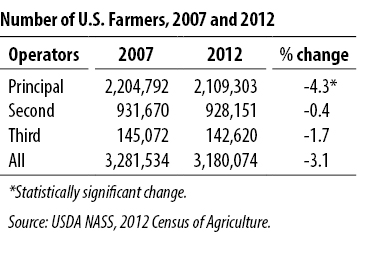
\includegraphics[width=.9\columnwidth]{project/images/fig1.png}
    \caption{The decline of US farmers \cite{census2012}.}
\end{figure}

\begin{figure}
    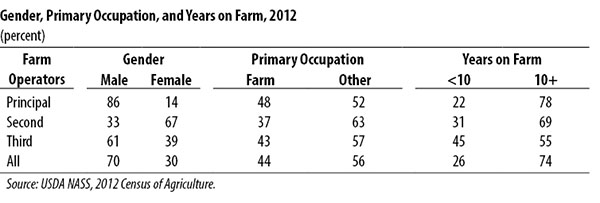
\includegraphics[width=.9\columnwidth]{project/images/fig2.png}
    \caption{Farm occupation statistics \cite{census2012}.}
\end{figure}

Being able to produce food within urban areas is a dynamic approach to helping solve several problems. This process of growing food and other greenery in urban areas would not only help ease the demand for food from sources outside the urban areas, but it also helps to create less of an environmental impact while simultaneously promoting a sustainable model. By again causing even less strain on the farming resources outside of the urban sectors, this enables them to focus on a more manageable demand \cite{landry2014}. Growing what is needed locally within urban areas is a great way to help the environment, increase availability while also providing food and agricultural goods for a growing population, and encourage a sustainable agricultural model. One major benefit of farming in a close system like an urban farm is that since the system is closed, the urban farmers do not have to worry about insects, rodents, or other pest infestations that might destroy their crops. But more importantly, the nature of the closed system means they do not have to used insecticides, pesticides, or rodenticides. This means the urban crops are safer for consumption and that they leave a much smaller environmental foot print than their rural cousins \cite{landry2014}. This closed system method also allows the urban farmers to use the precise amount of resources that their data indicates they should be using to grow their plants. This increase in efficiency is not only an economic boost, but further improves this model of sustainability by making the environmental footprint of farming even smaller. Data science is also helping improve these endeavours in the same way it helped with farmers in the mid to late 20th century: by applying rigorously tested computing models to agricultural jobs, urban farmers are pushing the envelope in regards to how much food they can grow with limited spaces while saving on resources \cite{auernhammer2001}. 

The United States and other developed nations are not the only places taking advantage of these advances in farming technology, newly developed processes for improving production, and taking advantage of agriculture data analysis. Developing nations are also benefiting from this new era where agriculture is meeting modern technology. As world populations grow and nations develop further, the demand for more and varied goods increases, including a demand for more varied foods. By taking advantage of data science practices, farmers and food providers in developing nations are discovering new and innovative ways to meet this new demand placed on them for their goods. These new approaches are helping developed nations two fold: not only are they helping farmers to produce greater and more varied quantities of food, but they are also helping to limit the environmental footprint, created from farming, in places that are more sensitive to environmental change, or where environmental laws are not as heavily enforced \cite{garnett2013}. The ability to meet food demands, curtail the effects of climate change on the surrounding environment, maximize the efficiency of resource use, and take advantage of advances in food storage and distribution are helping to transform developing nations in ways that all of their citizens can benefit from. Limiting and reducing the environmental footprint of farming and other agriculture processes is also extremely beneficial for developing countries and places that are facing more extreme, contemporary threats from climate change, as opposed to other nations whose economies and well being are less dependent upon their agriculture sector \cite{garnett2013}. The direction that modern farmers in developing nations are taking, and their focus on sustainability, are only possible because data analysis tools have brought the world's agricultural expertise to this point. Keeping the data open and friendly allows for cross applicability of the data, which leads to more insights and discoveries, which in turn continues to benefit the farmers and agriculturalists even more.

\subsection{Focusing On Sustainability}

As mentioned previously, the growing focus on sustainability is helping to drive technological innovation and advancements and new techniques that produce more and better food while also limiting and reducing the environmental footprint required to do so. This is good news for farmers who are facing a shrinking population of agricultural workers in the face of growing demand for food in centralized urban areas. This growing demand has not gone unnoticed by the governments of the world, and many of them are actively taking steps by working with farmers and providing resources for research and development of farming practices that leave the ones farmers have been using in the dust. This focus on sustainability is not just for places like the United States who have the resources to explore new and dynamic avenues for agricultural experimentation. These new techniques and processes are also being quickly adopted by developing nations around the world in order to combat their countries' own hunger and resource problems. With the looming threat of climate change, whose impact is already beginning to make itself more and more apparent around the world, the demand and pursuit of data oriented precision agriculture is increasing at an exponential rate \cite{trauger2009}. Since the well being of many developing nations is tied so closely with their agricultural production, they are the most susceptible to climate changes and the damage it can cause to food production \cite{mendelsohn1999}. Humanity is good at overcoming adversity, however, and data science is clearly helping to tackle the effects of climate change on agricultural endeavours and food production. The threat of climate change itself is driving entirely new agricultural fields whose sole focus is on sustainability.

There are many factors driving the technological innovation in data science focused agriculture. But of all of them, human caused climate change is perhaps one of the biggest factors driving the changes and modern focus on sustainability, especially in developing nations. ``Because most developing countries depend heavily on agriculture, the effects of global warming on productive croplands are likely to threaten both the welfare of the population and the economic development of the countries'' \cite{mendelsohn1999}. Since developing nations are more sensitive to the effects of climate change because their economies and well being are often directly dependent on their agriculture sector, they are the ones who are benefiting the most from all the advancements in this field. These benefits are having a stabilizing effect in areas where theses practices are being used, allowing for these places to develop further in areas that they ordinarily would not be able to focus on if they were still struggling to meet food requirements. By being able to focus on other parts of their society, these nations are able to further develop themselves and achieve greater and greater standards of living and freedoms for their citizens \cite{lee2005}. This is just one example of how agricultural data science has positive effects on society outside of the agricultural and environmental sectors. These effects, when used with noble intentions, are good for everyone.

\subsection{Urban and Vertical Farming}

As touched upon briefly earlier, when farmers begin producing some of the fruits and vegetables that people need inside of urban areas instead of on farmlands, this helps ease another one of the biggest problems farmers have encountered in the past, the problem of land availability. Again, as populations continue to grow, the stress they put on the demand for resources becomes more and more extreme. Land and resources becomes more and more scarce, not only because they are required for people to live on, but also because lots of other resources are required to handle large populations. Land resources for building roads for transportation, food and retail zones, resources such as land fills, waste removal, hazardous storage, water treatment, and power plants are just a few of the many other land resource demands that increase hand-in-hand as urban populations increase. One novel solution being used by many countries to tackle the problem of scarce geographic resources comes from thinking dynamically about the problem and realizing that, technically, farmland is not required in order to grow food and have a farm. Instead of expanding outward in order to grow more food, some modern farms are being rethought and built upwards or in repurposed, closed and controlled facilities in major urban areas. By utilizing or building multi-level structures laid out over a semi large area, farmers are able to grow different crops at different levels. These installations can be built in major urban areas, but any open urban space will do. This has the bonus side effect of reusing old buildings that might not have previously been in use anymore, which adds to and promotes a sustainable model. These structures allow for the same kind of closed system farming techniques that precision farming benefits from, while also allowing farmers to control everything that is done to their crops \cite{despommier2013}. Having all the plants in urban areas also has the benefit of naturally cleaning the air. Plants use many of the gases released in vehicle emissions for their life functions. Taking these harmful gases out of the air is beneficial to humans, the plants, and the surrounding environment \cite{despommier2013}. Building urban farms like this is a win for everyone involved, and as people and governments begin to take a more active role in regards to improving and pursuing sustainable models of food production and environmental protection, urban farms are likely to gain in popularity and start popping up all around the world.

Another angle that can be taken in regards to vertical farming is the idea of growing plants on all available flat surfaces. Not only floors, but also ceilings and walls where available. One problem major urban areas can have is a lack of green spaces available. This takes away from the aesthetics of these urban locations, while also allowing for pollution to go to choke out major areas in cities. Growing plants on some walls and buildings around major cities will help reduce the impact of both of these problems on the people and their environment. The plants being around the city take care of the lack of green places on its own, transforming concrete jungles into lush, semi-green cities. Meanwhile, the plants themselves will help clean up pollutants in the air from human emissions and simultaneously reduce amounts of noise pollution in their immediate vicinity. These green walls can even be limited to urban agricultural buildings themselves and would still be effective and have a positive impact on their immediate environment \cite{suparwoko2017} Again, data science makes all of this possible by allowing analysts and farmers to figure out the best ways to execute their agricultural endeavours, how to grow their plants, which and how much of their resources they need to use, and so forth. Technically, all of this could have and has been done in the past; it is not difficult to grow plants on the sides of buildings. But now urban populations are reaching heights that have never been seen, and the demand on environmental resources and human emissions are ever increasing. These simple approaches to the problems presented above are a means for cities to tackle a lot of the problems in city living, along with helping ease their dependency on farmlands for resources \cite{suparwoko2017}. When urban farmers and city planners have access to data science and analysis tools that allow them to review and analyze information at a much deeper level, they are able to find new insights into the problems they are trying to solve. These new insights are driving urban farming to the level it needs to be at in order to meet the needs of an ever growing population and increased urban demand on resources.

\subsection{Precision Farming: Networked Farms}

The idea of a connected farm is paramount in moving beyond the historical approach to farming and agriculture. The cornerstone of understanding and finding better techniques to improve farming is data, and a networked, or smart farm, does just that. By using technology that networks the farmland, the farmer now has access to a decisions support network, which allows farmers the ability to keep track of all the happenings taking place on their property in ways they have not been able to in the past. This new attention to detail taking place allows farmers and agriculturalists to engage in a practice called precision agriculture. Precision agriculture ``concentrates on providing the means for observing, assessing, and controlling agricultural practices'' \cite{kassim2014}. In essence, precision agriculture, or smart farming, focuses on sustainability and finding the sweet spot between resource use and crop growth and food production. Being able to hit that efficiency spot allows farmers to save on resource use while getting the most bang for their buck in regards to crops grown and sold per acre. Farmers are able to take advantage of all kinds of new data at their disposal. They have access to modern technology, which allows them access to things like satellite telemetry data on not only the weather, but also insect populations and blooms, as well as a myriad of data on other farming techniques and practices that are still evolving to improve efficiency and production.

By taking advantage of new technology, as well as Internet of Things based technology, farmers and agriculturalists are able to tap into a source that humans have never been able to use in the past. Examples of modern agricultural technology include advances in wireless sensor technology that allow for the monitoring and changes in environmental conditions, resource use and precision agriculture, warehouse and storage management for storing crops and other perishables, technology that allows for large amounts of automation, and RFID technology that allows for tracking of the distribution of goods from farms \cite{wang2006}. All of these new technologies work in conjunction with one another to improve all aspects of the farm by making it possible to accurately monitor for and detect small problems that might arise and get them taken care of before they turn in to big problems. This proactive process of monitoring for problems fits with the growing importance of sustainability. Getting to problems and fixing them before they become larger issues can help the farm in countless ways. Practical ways in which data science technology can help improve farms are detecting insects, rodents, or other pests before they become an infestation, monitoring environmental conditions outside or in storage spaces in order to ensure that the crops they have stay fresh longer and do not become tainted in any way, determining the precise amount of resources required for individual plots of land or crops being grown so the farm's resources are being used more efficiently, soil analysis to determine the best kinds of plant strains for their specific farmland, and tracking the distribution of their farm goods in order to more accurately distribute them to retailers. All of these agricultural techniques come together to form the larger picture that shows how much data science has really changed the agriculture sector. All of these technologies only came into existence in the last 25 years \cite{wang2006}.

\begin{figure}
    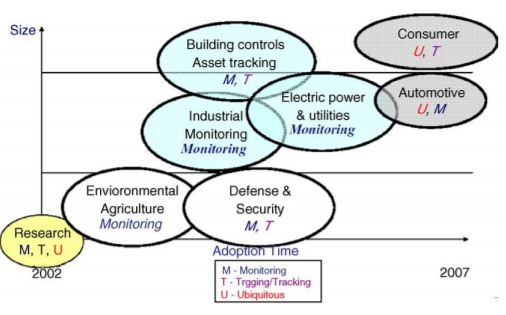
\includegraphics[width=.9\columnwidth]{project/images/fig3.png}
    \caption{Projections show how quickly the technology was growing at the start of the 21st century \cite{wang2006}.}
\end{figure}

\subsection{Modern Agricultural Data Science Beyond Food}

Data science has the power to improve farming and agriculture in ways beyond just precision agriculture and growing food in ways and places that have never been done before. By taking a look at the entire picture, it is possible to shave even more off the proverbial top in terms of efficiency and improving sustainability in relation to farming and agriculture. Data science can improve the economic returns of local farmers while also helping to minimize the environmental footprint that is produced from the production and transportation of goods. Modern technology and machines enable for the harvesting, gathering, and preparation of food goods to be automated, faster, and much more efficient than if it was done by hand \cite{wang2006}. Modern technology also allows for the farmer and business owners to keep track of how much of their products are being sold and in which locations. This allows the retailer to order more precise amounts to fit their needs while also informing the farmer which crops are best to grow, when to grow them, and what quantities to shoot for. GPS and other transportation technology can be used in the transportation process to make sure that the drivers have the most direct and efficient routes possible while delivering their goods, and advances in communications technology make it easy for orders to be changed or updated at the last minute \cite{trauger2009}. The goal of all of this is to produce less overall waste and put less stress on the environment. Data science helps mitigate problems that would produce more waste and add stress to the environment, so in this way, it is one of the most important tools humanity has in solving these problems and continually improving the agriculture sector to meet the demands of bigger populations.

\subsection{Setbacks and Steps Towards the Future}

The ability to analyze agriculture data with modern technology is leading to many unexpected discoveries. With sustainability and combating climate change being two of the most important driving factors in innovation, scientists and farmers and finding are using data science models to find dynamic solutions to problems, both old and new. At this point one of the biggest problems holding back agricultural data science, despite the fact that more and more data is being generated everyday, is the distinct lack of data. There are many challenges that must be overcome as we move towards the future of agriculture, but one of the greatest obstacles ``is to obtain reliable data on farm management decision making, both for current conditions and under scenarios of changed bio-physical and socio-economic conditions'' \cite{capalbo2017}. In other words, it is not a question of having reliable data, as much as it is a question of having reliable data that pertains to scenarios and circumstances that are difficult to reproduce, that have not happened yet, but are speculated to happen as the climate change. Despite this, the modern data that has been collected is obviously still being put to good use and helping to solve major problems that humanity knows will be immense obstacles in the future.

One example of a modern solution to an old problem is fighting emissions that pollute the earth. Although it is often thought that vehicle and airplane emissions cause the most air pollution, but of all of humankind's endeavours, it is factory farming that is having the biggest impact on our environment and exacerbating the effects of climate change \cite{caro2014}. Agricultural data science is being used to help combat the effects of factory farming in a number of unorthodox ways. One recent example of agricultural data science making a breakthrough in this area came when scientists discovered that feeding cows, who are by far the biggest producers of methane and other remissions, ground up bits of seaweed with their regular feed will radically reduce the amount of methane they produce while having no negative affect on the animals \cite{kinley2016}. The wireless monitoring sensors and models used to ascertain these findings were only available because they were created from investments in the pursuit of agricultural data science practices. As findings like this become more common and see widespread adoption, the environmental footprint of factoring farming will begin to decline. This will be incredibly useful for developed nations whose factoring farming emissions levels are continuing to rise \cite{caro2014}.

\begin{figure}
    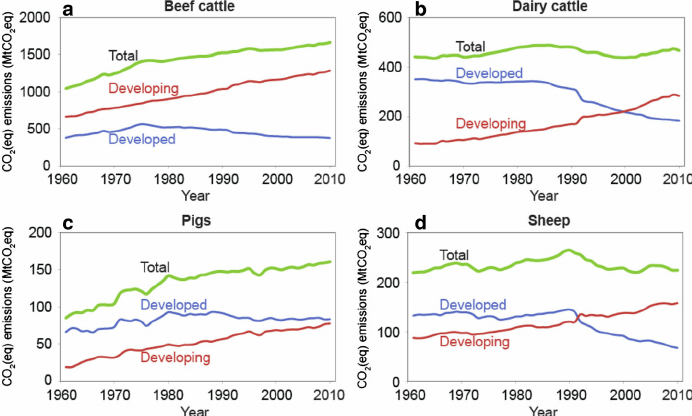
\includegraphics[width=.9\columnwidth]{project/images/fig4.png}
    \caption{Cattle emissions rate trends over the years \cite{caro2014}.}
\end{figure}

\section{The Future of Agricultural Data Science}

The future of agricultural data science is concerning itself with not only continuing to solve and improve the same old problems, but also exploring entirely new, out of this world concepts in regards to farming and growing foods. In the past, agricultural data science was focused on gathering data and growing the field. Modern agricultural data scientists are taking on problems like climate change, staggering populations and their demand for food, and finding new ways to improve sustainable agricultural models. So, then, it seems that the future of agricultural data science is beginning to come into focus. Although new problems and fields are bound to arise, the focus of the future of agricultural data science seems to be on automation and enhanced sustainability through disturbing the environment as little as possible \cite{kassler2001}. Since machines are able to perform tasks more efficiently that humans can, reaching a point of agricultural automation is one of the potential goals of sustainable models. A mostly automated farm is much more efficient that one that relies on the human element to perform jobs and work. That is not to say that there will never be a human element involved, but the future farmers may have more in common with data scientists and programmers than they do with their modern and historical counterparts who worked in fields most of the day \cite{purdy2016}. As technology improves in ways we cannot imagine right now, the possibilities of how data science will influence agriculture in the future are great.

The future may seem like science fiction in many ways, but modern technology and agricultural procedures may have seemed like science fiction if they were explained to a farmer from the 1950s. That does not mean that we are not able to see where a lot of different areas or advancing, to theorize technology and procedures that farmers and agriculturalists are not able to take advantage of now because they are too expensive. But as technology becomes cheaper and new methods and data science models are built, the future quickly becomes the present as humans catch up with their imaginations. Advances in automation, bloodless food production, extra-solar farming, and eventually terraforming, when realized, have the potential to transform our society in astonishing ways, possibly even leading to a post scarcity society where everyone's basic needs are met. Where agriculture itself enabled humankind to stop focusing on strictly survival and evolve into societies, so too might automated agriculture and food production allow for humanity to achieve a new level of societal evolution \cite{david2017}.

The coming changes in agricultural data science are not simply limited to technological or physical. Indeed, even now as humanity's understanding of its impact on the climate and surrounding environment is coming to be better understood, world governments are beginning to realize the important of sustainability and limiting the environmental footprint that is created from food production. World governments taking an active interest is having a positive effect on the research and development being done in the fields related to agricultural data science \cite{capalbo2017}. This new emphasis is changing the way many politicians think about agriculture and making them eager to use political leverage to enact changes in government which put guidelines into place and make resources available that enable agricultural researches to analyze their data and make informed decisions when attempting new agricultural endeavours. 

\subsection{The Future and Automation}

Much as sustainability and environmental impact are big tent poles driving innovation in agricultural data science and technology, so too will they continue to be in the future. However, a third piece of the puzzle is being thought of as more data is generated an analyzed, and that piece is automation. Automation is when technology and machines work to perform the jobs and tasks that humans would ordinarily do. Automation makes work far more efficient because, typically, a machine requires less resources to perform work than a human does. The resources a machine requires come largely in the form of costs upfront, but they quickly pay for themselves \cite{kassler2001}. Automation allows for producers to produce their product around the clock, so too would the crops on an automated farm receive constant care and attention that a human would be unable to provide. This fine attention to detail would increase the amount of food produced and improve resource use efficiency for growing food.

This concept is not referring to an enormous, single intelligent farm that knows all. Instead, an automated smart farm would actually be a collection of many smaller, automated systems that all work together to ensure the success of the farm and its food production requirements. Not all farms would need to be completely autonomous in order to benefit from this technology. For example, some farms are already taking advantage of available to technology to automate simple tasks and jobs that humans used to perform, such as automated irrigation systems \cite{gutierrez2014} and tools that automatically extract key data bits from current crop conditions and executes automated commands to tend the farm, based on a set of predefined variables \cite{das2015}. Nonetheless, as more and more automated systems are made available and become less expensive, more farms will be adopting them, leading to an even greater level of automation and requiring even fewer workers with diverse skill sets than ever before.

\subsection{Meat Grown in Labs}

Climate change is one of the biggest threats spurring research and interest in efforts to improve sustainable agriculture practices. As mentioned earlier, the one human activity that by far has the greatest impact on the environment is factory farming, which is a process of raising cattle and other livestock in controlled conditions \cite{caro2014}. Similar in approach to precision agriculture, factory farming in developed nations is having a substantial impact on the environment from all the emissions the animals produce, as well as the resources that are required to operate factory farming facilities. This poses a problem for future generations since it is an unsustainable model. One solution being aided by data science that is currently too expense is the possibility of growing meat in a laboratory setting without requiring the growing and slaughtering of actual animals. Basically, this process is ``a novel idea of producing meat without involving animals with the help of tissue engineering techniques'' \cite{bhat2015}. At present levels of technology, this process is possible but far too expensive to be a practical solution to producing food on a large scale. However, data science models are helping to drive down costs by allowing scientists to analyze their data and find more efficient ways to accomplish their goals. Once it becomes less expensive to grow meat in a lab that is indistinguishable from traditional meat, protein farms will likely start popping up all over the world \cite{bhat2015}.

There are other benefits to think about when considering the impact of switching from traditional meat production to lab grown. The biggest, as mentioned slightly above, is that it will help to dramatically reduce the environmental footprint being created by factory farming practices. Growing meat in labs, once costs and techniques are worked out, has the potential to be radically more sustainable model than humankind's current practices \cite{heffernan2017}. Once it becomes possible and feasible to be able to grow all the healthy meat needed to satisfy the demands of the growing population in a labs, this model will begin to be adopted because of the economic and environmental advantages to its use that come with following a model focused on sustainability. Data science is helping to make this more of a reality by producing more advanced models that help scientists and engineers get their jobs done and find newer, cheaper ways to produce this lab grown meat \cite{heffernan2017}.

\begin{figure}
    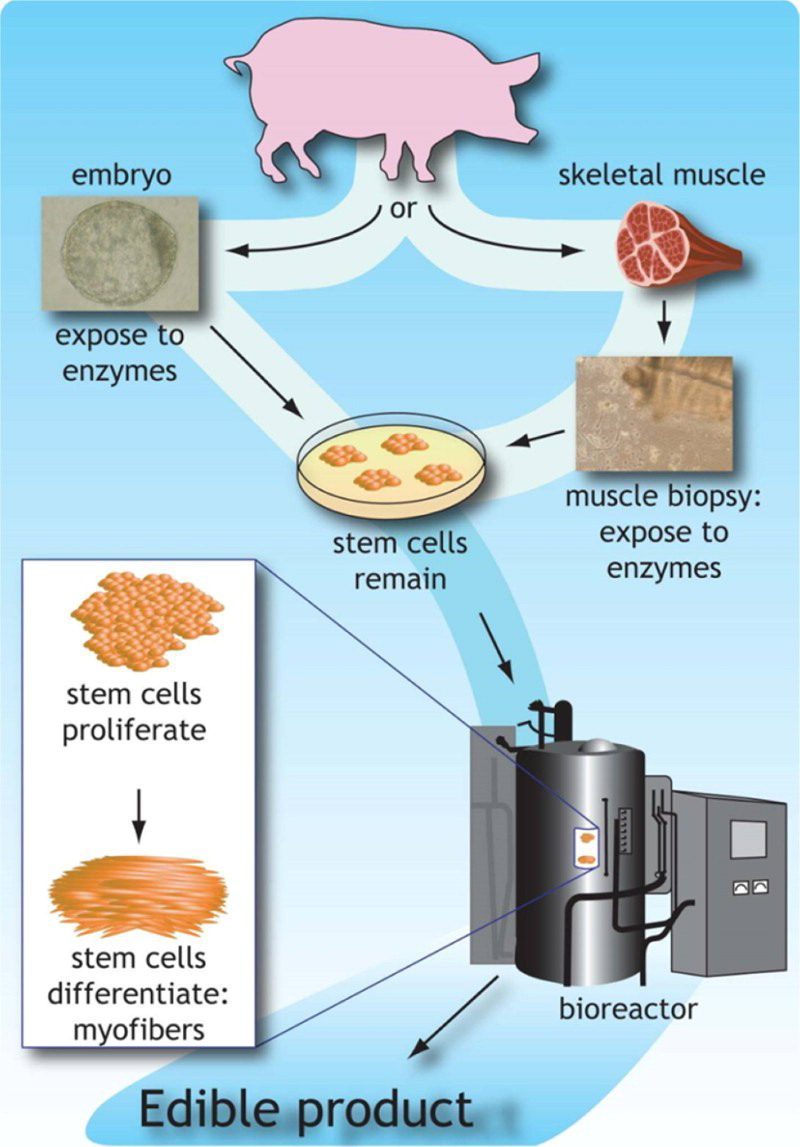
\includegraphics[width=.9\columnwidth]{project/images/fig5.png}
    \caption{Simplified process by which stem cells grow edible meat \cite{stephens2016}.}
\end{figure}

\subsection{Farming in Space}

One undeniable truth about humanity is that humans expanding and exploration seem to be hardwired into our genetic makeup. Since the beginning of humankind's history, exploration and settlement have been a big part of what drives human innovation. Necessity is the mother of invention, as the saying goes. It is in the spirit of that saying that future agricultural endeavours are being theorized and planned for today. One big possibility on the horizon is the necessity to grow food and farm off-world because of lack of space, resources, or environmental factors making the available farmland incapable of meeting the demands of future populations \cite{purdy2016}. Once agricultural development and food production reach a tipping point in regards to demands and human population, there will be no choice but to start farming in space. Enormous and fantastical space stations could be constructed where food could be grown in closed systems. This endeavour, though expensive, would eventually pay for itself and allow for a level of control, efficiency, and automation not available on Earth \cite{purdy2016}. By designing and constructing a station like this from the ground up, with things like sustainability and efficiency in mind, food will be able to be produced in a way never before practiced by humanity. This has the added benefit of having absolutely no impact on the environment, since it is not even being done on Earth. Right now, space travel and getting super structures like this built are prohibitively expensive. However, the costs of such things are expected to go down as technology advances and methods of space travel become more available \cite{viscio2014}.

\subsection{Terraforming Worlds: the Height of Agriculture}

At the most extreme end of outside the box thinking comes the most fantastic sounding concept yet: terraforming. Terraforming is the process of making another planet or heavenly body habitable for humans to live and thrive on. In the distant future there may come a time when humanity needs to take steps to become a multi-planet species. Data science will be invaluable when achieving this level of agricultural endeavour as the amount of data to be processed and understood will require data analysis models and techniques that have not even been invented yet \cite{dance2016}. The ability to adapt a planet to human life would require a complete mastery of agriculture which could only be obtained through refined understanding of unimaginably large amounts of data created from attempting such a task. Right now, scientists can only re-create extraterrestrial soil in a labs and perform experiments to grow food there, so any work done in this field is mostly hypothetical, but not outside the realm of possibility. If humans continue to advance at the exponential pace at which they are, one thing begins to become undeniable clear. Given a long enough timeline, environmental, societal, or geographical conditions will come about that will one day make it a necessity for humans to start living on multiple planets. Although this is science fiction now, data science and the insights its use grants us are making the impossible possible everyday.

One applicable experiment that was performed to test the validity of adapting the soil on Mars to growing terrestrial flora was when scientists looked at the recent volcanic iron deposits in Santorini, Greece. The bizarre lifeforms that were found living in this environment ``provides a potentially useful ecosystem for Mars terraforming experiments'' \cite{robbins2015}. Using data science to gather and make sense of the data generated on terrestrial locations that are similar to extraterrestrial ones brings humanity one step closer to terraforming, even if it is a baby step. As fantastical a concept as bending another planet to humanity's will is, if you stop to think about it, this is nothing new. Humans have been terraforming the Earth for thousands of years already, just not in the ways we would prefer. Terraforming on a large scale is theoretically possible, but it will never be possible without the data science tools and techniques to analyze the mountains of data that would be need to be analyzed to achieve such a advantageous goal that may one day be a neccesity.

\subsection{Restructuring Society}

The possibility of achieving a post-scarcity society, while seemingly outlandish considering humanity's current problems, could become a reality in the future. Having all of humanity's food needs met automatically through space aged inventions like massive orbiting space farms and home or lab grown meat would lead to a restructuring of society humans have not seen since we first started farming twelve thousand years ago \cite{david2017}. Should humanity ever achieve this level of societal progress, data science methods and models will be largely to thank for allowing humans to understand and improve their work by analyzing the data it produces. A largely automated society would produce an enormous amount of data to be analyzed, which as previously discussed, has the benefit of becoming even more sophisticated as more data is generated to learn from \cite{biem2015}. This self reinforcing system of generating data, improving from it, then generating more is showing no signs of slowing down as humanity is only just now beginning to see the benefits of complex automation. Self driving vehicles and automated farms are on the horizon, as well as a myriad of other technological innovations, and data science and its versatile applications are one of the biggest reasons that humanity has to thank for these technological possibilities.

\section{Conclusion}

Humanity's modest roots as simple nomads who discovered that they could grow their own food and use agriculture as a tool to build civilizations lasted for thousands and thousands of years. There were advancements, sure, but they were slow in coming and lacking in sophistication. However, in the last 75 years or so, humanity has seen the agriculture sector explode with new developments in techniques, technologies, and practices that have increased food production and allowed the agricultural sector to keep pace with growing populations that have a greater demand for food and agricultural resources. How was the agricultural sector able to revolutionize itself when in the past, changes came about much more slowly and incrementally? The answer, of course, is that the field of data science has been one of the chief tools used to solve agricultural problems and find solutions that meet the demands of today.

Technological advancements in hardware and modeling systems are ushering in a whole new era of human agriculture that focuses on sustainability. Producing as little waste as possible, while also impacting the environment in ways that contribute to climate change in as few of ways as they can are among the most important goals of modern day agriculture and food production, and data science is helping farmers and agriculturalists achieve these beefy goals. By creating vast networked farms, modern day farmers and agriculturalists have access to a level of data analysis that has not been available in the past, enabling them to make informed decisions and change the way they do things in order to improve the efficiency and output of their farms. This analysis is also leading to improved sustainability practices on farms by allowing the farmers to understand statistics about resource use and relation to crop growth like they could not in the past. Urban farming is also proving to be a modern solution to food distribution problems in highly populated areas, while also having the beneficial side effect of the plants helping to clean and detoxify the potentially harmful human made emissions that are found in major cities around the world.

The field of data science, from its origin to its current state as one of the premiere methods of human problem solving, is only going to continue to become more and more sophisticated as time goes on. With computer technology continuing to become smaller, cheaper, and more powerful, as well as data analysis models increasing in their reach and sophistication, the future of decision management tools and informed decision making that is going to be available to farmers and agricultural workers will be staggering. The future that agricultural data science is enabling seems like science fiction, but it is rapidly becoming a reality. Major projects like orbiting farms that meet the demands of the Earth's people to terraforming entire planets are going to require advanced tools and models that only sophisticated data science techniques and models will be able to provide in the future. Although humanity is still going through the growing pains of becoming a global, connected community, the future looks bright, statistically speaking. World hunger is still a problem humans are trying to solve, but data science has empowered us to fight it on a level battlefield where. Assuming human innovation continues at the exponential rate it has set for itself, the struggle to feed every human is a battle data science will help us to win.

\begin{acks}

The author would like to thank Dr. Gregor von Laszewski, Miao Jiang, and Juliette Zerick for assistance with my assignments and using github.

\end{acks}


\bibliographystyle{ACM-Reference-Format}
\bibliography{report} 



\section{Issues}

\DONE{Example of done item: Once you fix an item, change TODO to DONE}

\subsection{Assignment Submission Issues}

    \DONE{Do not make changes to your paper during grading, when your repository should be frozen.}

\subsection{Uncaught Bibliography Errors}

    \DONE{Missing bibliography file generated by JabRef}
    \DONE{Bibtex labels cannot have any spaces, \_ or \& in it}
    \DONE{Citations in text showing as [?]: this means either your report.bib is not up-to-date or there is a spelling error in the label of the item you want to cite, either in report.bib or in report.tex}

\subsection{Formatting}

    \DONE{Incorrect number of keywords or HID and i523 not included in the keywords}
    \DONE{Other formatting issues}

\subsection{Writing Errors}

    \DONE{Errors in title, e.g. capitalization}
    \DONE{Spelling errors}
    \DONE{Are you using {\em a} and {\em the} properly?}
    \DONE{Do not use phrases such as {\em shown in the Figure below}. Instead, use {\em as shown in Figure 3}, when referring to the 3rd figure}
    \DONE{Do not use the word {\em I} instead use {\em we} even if you are the sole author}
    \DONE{Do not use the phrase {\em In this paper/report we show} instead use {\em We show}. It is not important if this is a paper or a report and does not need to be mentioned}
    \DONE{If you want to say {\em and} do not use {\em \&} but use the word {\em and}}
    \DONE{Use a space after . , : }
    \DONE{When using a section command, the section title is not written in all-caps as format does this for you}\begin{verbatim}\section{Introduction} and NOT \section{INTRODUCTION} \end{verbatim}

\subsection{Citation Issues and Plagiarism}

    \DONE{It is your responsibility to make sure no plagiarism occurs. The instructions and resources were given in the class}
    \DONE{Claims made without citations provided}
    \DONE{Need to paraphrase long quotations (whole sentences or longer)}
    \DONE{Need to quote directly cited material}

\subsection{Character Errors}

    \DONE{Erroneous use of quotation marks, i.e. use ``quotes'' , instead of " "}
    \DONE{To emphasize a word, use {\em emphasize} and not ``quote''}
    \DONE{When using the characters \& \# \% \_  put a backslash before them so that they show up correctly}
    \DONE{Pasting and copying from the Web often results in non-ASCII characters to be used in your text, please remove them and replace accordingly. This is the case for quotes, dashes and all the other special characters.}
    \DONE{If you see a figure and not a figure in text you copied from a text that has the fi combined as a single character}

\subsection{Structural Issues}

    \DONE{Acknowledgement section missing}
    \DONE{Incorrect README file}
    \DONE{In case of a class and if you do a multi-author paper, you need to add an appendix describing who did what in the paper}
    \DONE{The paper has less than 2 pages of text, i.e. excluding images, tables and figures}
    \DONE{The paper has more than 6 pages of text, i.e. excluding images, tables and figures}
    \DONE{Do not artificially inflate your paper if you are below the page limit}

\subsection{Details about the Figures and Tables}

    \DONE{Capitalization errors in referring to captions, e.g. Figure 1, Table 2}
    \DONE{Do use {\em label} and {\em ref} to automatically create figure numbers}
    \DONE{Wrong placement of figure caption. They should be on the bottom of the figure}
    \DONE{Wrong placement of table caption. They should be on the top of the table}
    \DONE{Images submitted incorrectly. They should be in native format, e.g. .graffle, .pptx, .png, .jpg}
    \DONE{Do not submit eps images. Instead, convert them to PDF}

    \DONE{The image files must be in a single directory named "images"}
    \DONE{In case there is a powerpoint in the submission, the image must be exported as PDF}
    \DONE{Make the figures large enough so we can read the details. If needed make the figure over two columns}
    \DONE{Do not worry about the figure placement if they are at a different location than you think. Figures are allowed to float. For this class, you should place all figures at the end of the report.}
    \DONE{In case you copied a figure from another paper you need to ask for copyright permission. In case of a class paper, you must include a reference to the original in the caption}
    \DONE{Remove any figure that is not referred to explicitly in the text (As shown in Figure ..)}
    \DONE{Do not use textwidth as a parameter for includegraphics}
    \DONE{Figures should be reasonably sized and often you just need to
  add columnwidth} e.g. \begin{verbatim}/includegraphics[width=\columnwidth]{images/myimage.pdf}\end{verbatim}

re

\end{document}
